\chapter{Análisis crítico previo}

\section{Crítica}

Scrum vino a surgir como una alternativa al modo en que se desarrollaba software. Esta alternativa es presentada como posible solución a los problemas que presentaba la situación en ese entonces (década del 90) de Desarrollo de Software. Por esa razón es que por lo general cuando se habla de Scrum se hace un análisis crítico previo para plantear un cambio debido a un problema. Por un lado, Scrum plantea un cambio paradigmático que consiste en un cambio de perspectiva y de mentalidad (mindset). La otra cuestión fundamental es la metodológica en la cual se propone un cambio del proceso de desarrollo de software o proceso industrial de software. Por este motivo para comenzar a comprender Scrum hay que comprender cuál es el problema que viene a intentar resolver y qué es lo que se critica.

\section{Problema}

\section{Paradigma criticado}

\section{Metodología criticada}

La causa de los problemas y fracasos de los proyectos de software en la situación dada, en ese entonces, de Desarrollo fueron atribuidos principalmente a la Metodología Cascada (Waterfall Methodology) \cite{Ken-Schwaber-1995}. Pero hay que tener en cuenta de qué se habla cuando se critica a la metodología cascada. Pues la metodología cascada no es el modelo cascada y en ocaciones se han atribuido, en un sentido erróneo, las causas de los problemas al modelo cascada. Pues no se puede comparar Scrum con el modelo Cascada porque Scrum no es exactamente un modelo y ofrece soluciones a aspectos que el modelo cascada no ofrece. Aunque si, el modelo cascada, es perte de lo que se podría considerar una Metodología Cascada. 

\subsection{Modelo en Cascada}

El Modelo en Cascada (Waterfall Methodology) \cite{Ken-Schwaber-1995} es un Modelo Secuencial de Procesos para la ingeniería de software presentado por Winston Royce en 1970, aunque ya se venía desarrollando desde antes. Para algunos críticos, el Modelo en Cascada, se convirtió en el modelo metodológico más utilizado dentro de la industria en un período de tiempo. Pero hay que considerar que el modelo solo abarca al sistema de producción o sistema de desarrollo (ver "Development Process" en la figura \ref{fig:WaterfallMethodology}) de la industria y no al de gestión.

En un sentido lato y ortodoxo se puede decir que el Modelo en Cascada refleja un proceso lineal y secuencial de un conjunto de procesos o fases independientes dentro de un proyecto. Las fases son: requerimientos (requerimiento del sistema y requerimientos del software), diseño, codificación, pruebas y operación. Según esto y siempre cuando el proceso de desarrollo de un proyecto conste de solo la secuencia de estas fases sin repetición, la principales críticas como desventajas que se hacen son:

\begin{enumerate}

\item \textbf{Previción:} Al tener una face de requerimientos única al comienzo, el producto final es anticipado de antemano \cite{Scrum-Institute-2015}. Esto requiere de cierta previción y certidumbre inicial que en proyectos complejos y cambiantes es poco factible que suceda.

\item \textbf{Requerimientos no necesarios:} Requerimientos elicitados al comienzo del proyecto y luego implementados nunca serán completamente necesitados por el cliente \cite{Scrum-Institute-2015}. O sea que pueden haber requerimientos irrelevantes o inecesariamente implementados, ya sea porque el cliente dejó de tener la necesidad en el transcurso del proyecto o porque la incertidumbre inicial generó una mala elicitación de los mismos.

\item \textbf{Fases separadas:} Cada fase es estrictamente separada \cite{Scrum-Institute-2015}. Por ejemplo una vez que se encuentra completa la fase de requerimientos se procede a una firma de aprobación o "sign-off" que congela dichos requerimientos, y es recién aquí cuando se puede iniciar la fase de diseño, fase donde se crea un plano de modelo o "blueprint" del mismo para que, luego, los programadores lo codifiquen y se prosiga con las pruebas y finalmente el despliegue en operación. Pues en entornos altamente cambiante, propio de la industria de software, esta forma secuencial estricta hace del proceso de desarrollo un proceso “pesadas” (estanco y burocrático) y prohibitivo para responder satisfactoriamente a los factores cambiantes de negocio \cite{Martin-Alaimo-2014}.
%Solución propuesta por scrum:
%Fine-grained requirements are only defined when they are really needed.
%All activities to design, build and test a certain functionality are kept together in one phase.
%Changes are expected and welcomed by Scrum team.

\end{enumerate}

\subsection{Gestión de Proyectos Clásica}

\subsection{Metodología en Cascada}

\begin{figure}[h]
  \centering
  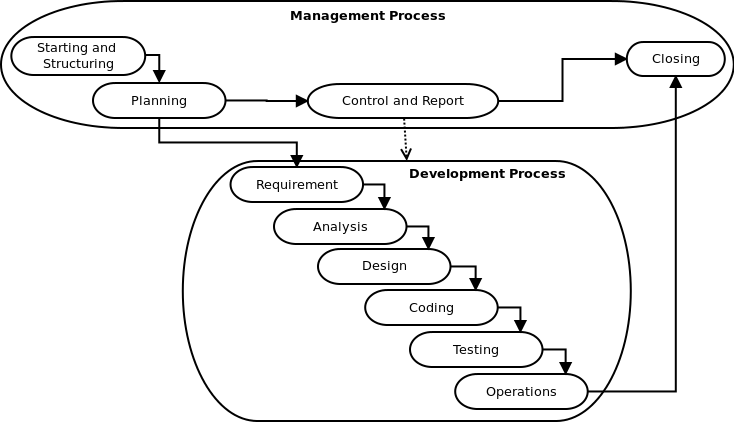
\includegraphics[scale=0.5]{WaterfallMethodology}
  \caption{Metodología Cascada criticada (Diagrama integrador del Modelo Cascada \cite{Winston-Royce-1970}, la Metodología Cascada \cite{Ken-Schwaber-1995} y la Metodología de Gestión de Proyectos \cite{PMBOK-1996})}
  \centering
  \label{fig:WaterfallMethodology} %\ref{fig:WaterfallMethodology}
\end{figure}
